\documentclass[11pt]{article}

% --- packages ---
\usepackage[margin=1in]{geometry}
\usepackage{amsmath,amssymb,amsfonts}
\usepackage{booktabs}
\usepackage{graphicx}
\usepackage{hyperref}
\usepackage{xcolor}
\usepackage{multirow}
\usepackage{float}
\usepackage[numbers]{natbib}
\usepackage{microtype}
\usepackage{bookmark}
\usepackage{tikz}
\usetikzlibrary{arrows.meta, positioning, fit, backgrounds}

\hypersetup{
  colorlinks=true,
  linkcolor=blue!60!black,
  citecolor=blue!60!black,
  urlcolor=blue!60!black
}

% --- metadata ---
\title{%
  Pesi strutturati sugli archi amplificano i vantaggi topologici\\
  del reticolo FCC tramite resilienza ai colli di bottiglia%
}

\author{%
  Timothy Paul Bielec\thanks{Autore corrispondente: \texttt{timothy@promptcrafted.com}}\\
  Promptcrafted LLC\\
  Los Angeles, CA
}

\date{Marzo 2026}

\begin{document}

\maketitle

% ===================================================================
\begin{abstract}
Un articolo complementare~\cite{bielec2026shape} ha stabilito che il
reticolo cubico a facce centrate (FCC) offre un vantaggio di
connettivit\`a algebrica pari a $2{,}3\times$ rispetto al reticolo
cubico semplice (SC) con pesi uniformi sugli archi. Il presente
articolo esamina se pesi strutturati sugli archi amplificano tale
vantaggio. Sette esperimenti condotti su due registri---tassellazione
a scala di reticolo e caratterizzazione a singola cella---rispondono
in modo definitivo: i pesi strutturati amplificano. La ponderazione
per direzione, motivata dalle sei coppie di facce del dodecaedro
rombico, porta il rapporto di Fiedler da $2{,}3\times$ a $6{,}1\times$
con 1\,000 nodi, confermato da un controllo per permutazione
($p = 0{,}001$ rispetto all'assegnazione permutata). Il meccanismo
\`e la resilienza ai colli di bottiglia: pesi eterogenei creano colli
di bottiglia prossimi alla disconnessione che i reticoli cubici non
riescono ad aggirare, ma i reticoli FCC s\`\i. A scala di singola
cella, una mappatura mirata primo-vertice raggiunge
$p \approx 2{,}5 \times 10^{-5}$ rispetto a un modello nullo esaustivo,
mentre l'analisi spettrale rivela che la soppressione del valore di
Fiedler con pesi del corpus si verifica in tutti i politopi a 24~archi
testati (percentili 0,02\%--5,94\%), suggerendo che l'effetto sia
determinato dalla distribuzione dei pesi piuttosto che dal grafo. Tutti
i risultati sono riproducibili tramite \texttt{rhombic} v0.3.0
(256~test, \texttt{seed=42}).
\end{abstract}

\noindent\textbf{Parole chiave:} topologia reticolare, grafi pesati,
connettivit\`a algebrica, resilienza ai colli di bottiglia, valore di
Fiedler, dodecaedro rombico, teoria spettrale dei grafi

\smallskip\noindent\textbf{MSC 2020:} 05C50 (primario), 05C22, 05C85, 52B10

% ===================================================================
\section{Introduzione}
\label{sec:intro}

\subsection{Contesto}

L'articolo complementare~\cite{bielec2026shape} ha confrontato le
topologie reticolari cubica semplice (SC, 6-connessa) e cubica a facce
centrate (FCC, 12-connessa) su quattro domini---teoria dei grafi,
operazioni spaziali, elaborazione del segnale e recupero per
embedding---trovando vantaggi stabili del reticolo FCC a tutte le
scale testate (125--8\,000 nodi). Il risultato principale \`e stato un
rapporto di connettivit\`a algebrica pari a $2{,}3$--$2{,}5\times$ con
pesi uniformi sugli archi: ogni arco ponderato in modo uguale.

Questa linea di base solleva una domanda immediata: cosa accade quando
gli archi hanno pesi diversi? I sistemi reali---reti neurali, catene
di approvvigionamento, reti di comunicazione, reticoli cristallini con
difetti---presentano intensit\`a di connessione eterogenee. Se i pesi
strutturati attenuano il vantaggio FCC, i risultati a peso uniforme
costituiscono un limite superiore di rilevanza pratica limitata. Se
invece lo amplificano, il vantaggio topologico \`e pi\`u robusto di
quanto suggerisca la linea di base.

Per riferimento, le metriche chiave dell'Articolo~1: i reticoli FCC
raggiungono cammini medi pi\`u corti del 30--32\%, diametro inferiore
del 40\% e un rapporto di Fiedler pari a $2{,}3$--$2{,}5\times$ con
pesi uniformi, stabili su 125--8\,000 nodi.

Il presente articolo riporta sette esperimenti che rispondono a questa
domanda. La Figura~\ref{fig:dependency} mostra la struttura di
dipendenza tra i due articoli e la gerarchia degli esperimenti
all'interno di questo.

\begin{figure}[ht]
\centering
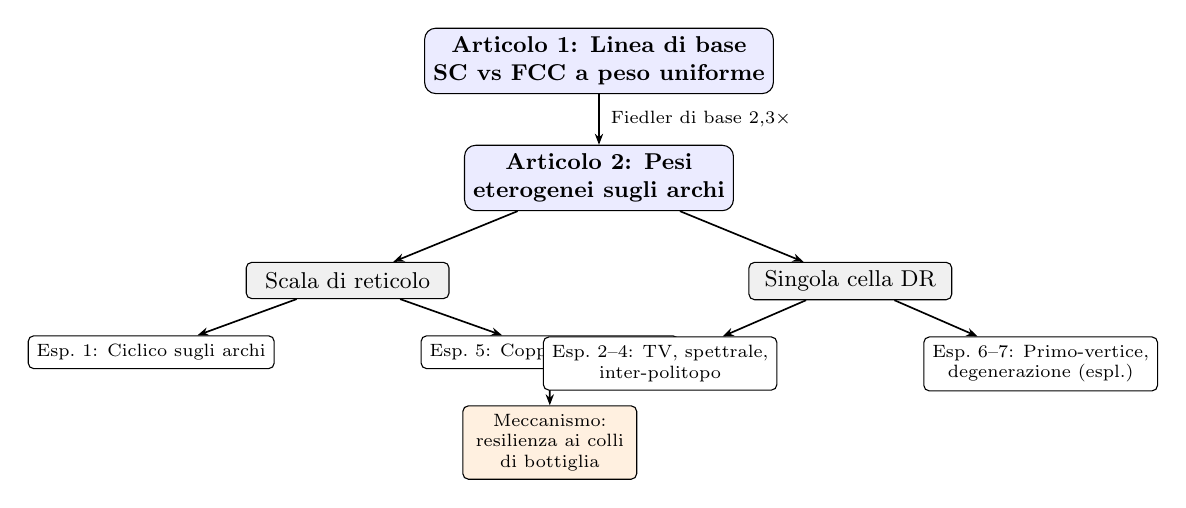
\begin{tikzpicture}[scale=0.92, transform shape,
  node distance=0.5cm and 0.6cm,
  paper/.style={draw, rounded corners, fill=blue!8, minimum width=3.5cm,
                minimum height=0.65cm, align=center, font=\small\bfseries},
  register/.style={draw, rounded corners=2pt, fill=gray!12, minimum width=2.8cm,
                   minimum height=0.5cm, align=center, font=\small},
  exp/.style={draw, rounded corners=2pt, fill=white, minimum width=2.4cm,
              minimum height=0.45cm, align=center, font=\scriptsize},
  mechanism/.style={draw, rounded corners=2pt, fill=orange!12, minimum width=2.4cm,
                    minimum height=0.45cm, align=center, font=\scriptsize},
  arr/.style={-{Stealth[length=4pt]}, semithick}
]
% Paper 1
\node[paper] (p1) {Articolo~1: Linea di base\\SC vs FCC a peso uniforme};

% Paper 2
\node[paper, below=0.7cm of p1] (p2) {Articolo~2: Pesi\\eterogenei sugli archi};

\draw[arr] (p1) -- node[right, font=\scriptsize, xshift=1pt]
  {Fiedler di base $2{,}3\times$} (p2);

% Two registers
\node[register, below left=0.7cm and 0.2cm of p2] (lat) {Scala di reticolo};
\node[register, below right=0.7cm and 0.2cm of p2] (cell) {Singola cella DR};

\draw[arr] (p2) -- (lat);
\draw[arr] (p2) -- (cell);

% Lattice experiments
\node[exp, below left=0.5cm and -0.4cm of lat] (e1) {Esp.~1: Ciclico sugli archi};
\node[exp, below right=0.5cm and -0.4cm of lat] (e5) {Esp.~5: Coppia di direzioni};

\draw[arr] (lat) -- (e1);
\draw[arr] (lat) -- (e5);

% Mechanism
\node[mechanism, below=0.5cm of e5] (mech) {Meccanismo:\\resilienza ai colli\\di bottiglia};
\draw[arr] (e5) -- (mech);

% Single-cell experiments
\node[exp, below left=0.5cm and -0.4cm of cell] (e234) {Esp.~2--4: TV, spettrale,\\inter-politopo};
\node[exp, below right=0.5cm and -0.4cm of cell] (e67) {Esp.~6--7: Primo-vertice,\\degenerazione (espl.)};

\draw[arr] (cell) -- (e234);
\draw[arr] (cell) -- (e67);
\end{tikzpicture}
\caption{Struttura di dipendenza. L'Articolo~1 stabilisce la linea di
  base FCC/SC a peso uniforme. Il presente articolo introduce pesi
  eterogenei su due registri: tassellazione a scala di reticolo
  (Esperimenti~1, 5) e caratterizzazione del singolo dodecaedro rombico
  (Esperimenti~2--4, 6--7). Gli Esperimenti~6--7 sono esplorativi.}
\label{fig:dependency}
\end{figure}

\subsection{Il corpus come insieme di pesi}
\label{sec:corpus}

Utilizziamo quattro distribuzioni di pesi sugli archi: \textbf{uniforme}
(tutti i pesi uguali), \textbf{casuale} (uniforme su $[0{,}1;\; 1{,}0]$),
\textbf{legge di potenza} (tipo Zipf: $1/\text{rango}$) e
\textbf{corpus}. La distribuzione corpus consiste di 24 interi
strutturati (intervallo 18--1\,296, media 318,8, deviazione standard
292,9) derivati da un protocollo di traslitterazione fisso applicato a
un insieme di 24 iscrizioni simboliche. Otto numeri primi
(11, 17, 19, 23, 29, 31, 67, 89) ricorrono come fattori nei valori
del corpus, conferendo alla distribuzione una struttura aritmetica
interna non banale. La provenienza del corpus e il suo significato
analitico sono documentati
separatamente~\cite{bielec2026shape}. Qui esso funge da test di stress
ad alta varianza e coda pesante, valutato insieme alle distribuzioni
uniforme, casuale e a legge di potenza.

Dopo la normalizzazione min-max a $[0,1]$, la distribuzione presenta
alta varianza (coefficiente di variazione $\approx 0{,}92$) e una
pesante coda destra (asimmetria $\approx 1{,}8$), propriet\`a condivise
con molte distribuzioni di pesi del mondo reale. Tutti i risultati a
scala di reticolo (amplificazione, resilienza ai colli di bottiglia)
possono essere verificati indipendentemente utilizzando le distribuzioni
casuale e a legge di potenza, che mostrano lo stesso gradiente di
amplificazione a magnitudine inferiore.

\subsection{Contributi}

\begin{enumerate}
  \item \textbf{Amplificazione:} I pesi strutturati sugli archi
    amplificano il vantaggio di connettivit\`a algebrica del reticolo
    FCC da $2{,}3\times$ (uniforme) a $6{,}1\times$ (corpus ponderato
    per direzione), pi\`u che raddoppiando la linea di base
    dell'Articolo~1.
  \item \textbf{Meccanismo:} L'amplificazione deriva dalla resilienza
    ai colli di bottiglia---la topologia 12-connessa dell'FCC aggira i
    colli di bottiglia prossimi alla disconnessione che limitano il
    reticolo cubico 6-connesso.
  \item \textbf{Coerenza inter-topologica:} La soppressione del valore
    di Fiedler con pesi del corpus si verifica in tutte e cinque le
    topologie a 24~archi testate (percentili 0,02\%--5,94\%),
    suggerendo che l'effetto sia determinato dalla distribuzione dei
    pesi piuttosto che dalla struttura specifica del grafo.
  \item \textbf{Coerenza primo-vertice (esplorativa):} Una mappatura
    mirata primo-vertice sul dodecaedro rombico raggiunge
    $p \approx 2{,}5 \times 10^{-5}$ rispetto a un modello nullo
    esaustivo di 40\,320 permutazioni.
\end{enumerate}

\paragraph{Organizzazione.}
La Sezione~\ref{sec:background} passa in rassegna la connettivit\`a
algebrica pesata e la struttura direzionale del reticolo FCC. La
Sezione~\ref{sec:method} descrive i due registri sperimentali e le
distribuzioni di pesi. La Sezione~\ref{sec:lattice} presenta gli
esperimenti a scala di reticolo (ciclico sugli archi e ponderato per
direzione), incluso il meccanismo di amplificazione. La
Sezione~\ref{sec:cell} presenta gli esperimenti di caratterizzazione
a singola cella (ottimizzazione TV, analisi spettrale, mappatura
primo-vertice, confronto inter-politopo). La
Sezione~\ref{sec:discussion} discute il meccanismo, i collegamenti
con la teoria della resilienza delle reti e le limitazioni. La
Sezione~\ref{sec:future} delinea il lavoro futuro. La
Sezione~\ref{sec:conclusion} conclude.

% ===================================================================
\section{Contesto teorico}
\label{sec:background}

\subsection{Connettivit\`a algebrica pesata}

La connettivit\`a algebrica di un grafo $G$ \`e il secondo pi\`u
piccolo autovalore $\lambda_2$ del laplaciano del grafo
$L = D - A$~\cite{fiedler1973}. Per grafi non pesati, Fiedler ha
dimostrato che $\lambda_2 > 0$ se e solo se $G$ \`e connesso, e che
un $\lambda_2$ maggiore implica una maggiore resistenza alla
disconnessione.

Per grafi pesati, il laplaciano pesato
$L_w = D_w - A_w$ si generalizza naturalmente: $(L_w)_{ij} = -w_{ij}$
per $i \neq j$, e $(L_w)_{ii} = \sum_j w_{ij}$, dove $w_{ij}$ \`e il
peso dell'arco $(i,j)$~\cite{mohar1991, chung1997}. Il valore di
Fiedler pesato $\lambda_2(L_w)$ \`e una misura spettrale della
vulnerabilit\`a ai colli di bottiglia. Disuguaglianze di tipo Cheeger
collegano $\lambda_2$ alla conduttanza del grafo---il rapporto minimo
tra il peso del taglio e il volume della partizione---ma $\lambda_2$
non \`e uguale al peso minimo del taglio~\cite{mohar1991, chung1997}.
La resistenza effettiva, la quantit\`a spettrale duale, misura quanto
bene un grafo distribuisce la corrente tra coppie di
nodi~\cite{ghosh2008resistance}; i grafi che massimizzano $\lambda_2$
minimizzano simultaneamente la resistenza effettiva nel caso peggiore.
La sparsificazione spettrale~\cite{spielman2004} preserva queste
propriet\`a spettrali in grafi ridotti, confermando che $\lambda_2$
cattura in modo robusto la connettivit\`a globale. Un $\lambda_2$
piccolo indica un collo di bottiglia a bassa conduttanza; un
$\lambda_2$ grande indica che non esiste alcuna partizione a basso
costo.

Quando i pesi degli archi sono eterogenei, $\lambda_2(L_w)$ \`e
dominato dal taglio pi\`u debole nel grafo. Una topologia con pi\`u
cammini alternativi attorno a qualsiasi taglio potenziale manterr\`a un
$\lambda_2$ pi\`u elevato sotto la stessa distribuzione di pesi.
Questo \`e il meccanismo che verifichiamo: il reticolo FCC fornisce 12
cammini per nodo rispetto ai 6 del cubico, e misuriamo se questa
ridondanza si compone sotto pesi eterogenei.

\subsection{Struttura direzionale nel reticolo FCC}

Ogni arco nel reticolo FCC connette vicini separati da uno dei 12
vettori di direzione
$\{\frac{1}{2}(\pm e_i \pm e_j) : i < j\}$. Queste 12 direzioni
formano 6 coppie antipodali, ciascuna corrispondente a due facce
opposte della cella di Voronoi (il dodecaedro rombico). Nel reticolo
SC, 3 coppie di direzioni corrispondono alle 3 coppie di facce del
cubo.

La ponderazione per direzione assegna lo stesso peso a tutti gli archi
che condividono una coppia di direzioni. Per l'FCC, questo mappa 24
valori del corpus in 6 coppie di direzioni (4 valori per coppia,
mediati); per l'SC, 3 coppie di direzioni (8 valori per coppia).
Questa assegnazione \`e motivata strutturalmente: riflette il fatto
geometrico che le 12 facce del dodecaedro rombico si presentano in 6
coppie parallele, creando 6 ``canali'' attraverso il reticolo con
intensit\`a regolabile indipendentemente.

% ===================================================================
\section{Metodologia}
\label{sec:method}

\subsection{Due registri: scala di reticolo e singola cella}

I sette esperimenti si suddividono in due registri.

\textbf{Scala di reticolo} (Esperimenti~1 e 5): reticoli FCC e SC
costruiti con conteggi di nodi corrispondenti (125--8\,000 nodi), con
archi pesati. Metriche: valore di Fiedler pesato, cammino minimo medio
pesato, velocit\`a di diffusione, convergenza al consenso.

\textbf{Singola cella} (Esperimenti~2--4, 6--7): il dodecaedro rombico
come singolo grafo (14 vertici, 24 archi), con valori del corpus
assegnati agli archi. Metriche: variazione totale sotto assegnazione
ottimale, propriet\`a spettrali, coerenza primo-vertice, confronto
inter-politopo.

Gli esperimenti a scala di reticolo misurano come topologia e pesi
interagiscono a scala di sistema. Gli esperimenti a singola cella
caratterizzano l'effetto dei valori del corpus sulla cella di Voronoi
stessa.

\subsection{Distribuzioni di pesi}

Quattro distribuzioni su 24 archi, tutte normalizzate a $[0,1]$:

\begin{itemize}
  \item \textbf{Uniforme:} $w_i = 1{,}0$ per ogni $i$.
  \item \textbf{Casuale:} $w_i \sim \mathcal{U}(0{,}1;\; 1{,}0)$, seed 42.
  \item \textbf{Legge di potenza:} $w_i = 1/\text{rango}(i)$, tipo Zipf.
  \item \textbf{Corpus:} 24 interi strutturati, normalizzati min-max.
\end{itemize}

A scala di reticolo, i pesi sono assegnati agli archi ciclando sulla
distribuzione a 24 elementi (Esperimento~1) oppure tramite media per
coppia di direzioni (Esperimento~5). A scala di singola cella, tutti
i 24 valori corrispondono direttamente ai 24 archi del dodecaedro
rombico.

\subsection{Ponderazione per direzione}

Per la ponderazione per direzione (Esperimento~5), i 24 valori del
corpus sono ordinati e partizionati in gruppi corrispondenti al numero
di coppie di direzioni: 6 gruppi di 4 per l'FCC, 3 gruppi di 8 per
l'SC. La media di ciascun gruppo diventa il peso per tutti gli archi
nella rispettiva coppia di direzioni. Ci\`o preserva la struttura di
varianza del corpus rispettando la simmetria direzionale del reticolo.

\subsection{Convenzioni sui rapporti}

Tutte le metriche comparative sono riportate come rapporti con direzione
esplicita. Le \textbf{metriche di livello} (valore di Fiedler, lunghezza
del cammino) sono riportate come FCC/SC: valori ${>}\,1$ indicano
maggiore connettivit\`a FCC; valori ${<}\,1$ indicano cammini FCC pi\`u
corti. Le \textbf{metriche di velocit\`a} (cicli di diffusione, cicli di
consenso) sono riportate come accelerazione SC/FCC: valori ${>}\,1$
indicano che l'FCC converge in meno cicli. L'intestazione di ciascuna
tabella ribadisce la propria convenzione.

\subsection{Definizioni delle dinamiche}

\textbf{Diffusione.} L'informazione si propaga tramite propagazione del
massimo con decadimento: a ogni ciclo,
$s_i(t{+}1) = \max\bigl(s_i(t),\; 0{,}9 \cdot \max_{j \in N(i)} s_j(t)\bigr)$.
Un singolo nodo sorgente parte a $s_0 = 1{,}0$; tutti gli altri a~$0$.
La copertura \`e la frazione di nodi che supera la soglia~$0{,}01$.
La metrica riportata \`e il numero di cicli per raggiungere il 50\%
di copertura.

\textbf{Consenso.} Tutti i nodi partono con stati casuali i.i.d.\
uniformi. A ogni ciclo,
$s_i(t{+}1) = \bigl(s_i(t) + \sum_{j \in N(i)} s_j(t)\bigr) / (\deg(i) + 1)$.
La convergenza \`e dichiarata quando
$\max_i |s_i(t) - \bar{s}| < \epsilon$ con $\epsilon = 0{,}05$,
fino a 500 cicli. Il denominatore $(\deg(i) + 1)$ include lo stato
proprio del nodo, producendo una diluizione per vicino a grado
elevato---il meccanismo alla base dell'inversione del consenso a
scala~1\,000.

\subsection{Software e riproducibilit\`a}

Tutti gli esperimenti utilizzano la libreria \texttt{rhombic}
(Python 3.10+, dipendenze: NumPy, NetworkX, SciPy). L'intera suite
sperimentale si riproduce tramite:
\begin{verbatim}
  cd rhombic && python scripts/run_experiments.py
\end{verbatim}
Tutte le operazioni stocastiche utilizzano \texttt{seed=42}. Tutti i
$p$-value sono calcolati come $p = (\text{numero di punteggi nulli} \geq
\text{osservato}) / N_{\text{nullo}}$. Quando nessuna prova nulla
supera il valore osservato, riportiamo $p \leq 1/N_{\text{nullo}}$.
Hardware: Windows~11, CPU Intel, NVIDIA RTX 6000 Ada 48\,GB
(inutilizzata---tutti i benchmark sono limitati dalla CPU). 256 test
verificano la correttezza della libreria. Il codice sorgente e i
risultati grezzi sono disponibili pubblicamente (si veda la
Sezione~\ref{sec:conclusion}).

% ===================================================================
\section{Esperimenti a scala di reticolo}
\label{sec:lattice}

\subsection{Esperimento 1: Benchmark pesati con ciclaggio sugli archi}

La distribuzione di pesi a 24 elementi viene ciclata su tutti gli archi
del reticolo. La Tabella~\ref{tab:exp1} riporta il rapporto di Fiedler
(FCC/SC) e il rapporto del cammino minimo medio (FCC/SC, pi\`u basso
\`e meglio) a tre scale.

\begin{table}[H]
\centering
\caption{Benchmark pesati con ciclaggio sugli archi. Rapporto di
  Fiedler = connettivit\`a algebrica FCC/SC ($>$1 = vantaggio FCC).
  Rapporto del cammino = cammino minimo medio FCC/SC ($<$1 = vantaggio
  FCC).}
\label{tab:exp1}
\begin{tabular}{llrr}
\toprule
Scala & Distribuzione & Rapporto di Fiedler & Rapporto del cammino \\
\midrule
125  & uniforme   & 2,31 & 0,69 \\
125  & casuale    & 2,49 & 0,66 \\
125  & legge di potenza & 2,67 & 0,67 \\
125  & \textbf{corpus} & \textbf{3,17} & \textbf{0,48} \\
\midrule
1\,000  & uniforme   & 2,55 & 0,68 \\
1\,000  & casuale    & 2,64 & 0,60 \\
1\,000  & legge di potenza & 3,06 & 0,64 \\
1\,000  & \textbf{corpus} & \textbf{3,11} & \textbf{0,39} \\
\midrule
8\,000  & uniforme   & 2,28 & --- \\
8\,000  & \textbf{corpus} & \textbf{3,18} & --- \\
\bottomrule
\end{tabular}
\end{table}

Il rapporto di Fiedler cresce monotonicamente con l'eterogeneit\`a dei
pesi: da 2,31 (uniforme) attraverso 2,49 (casuale) e 2,67 (legge di
potenza) fino a 3,17 (corpus) a scala 125. L'andamento \`e stabile
attraverso le scale. Il rapporto del cammino mostra lo stesso
gradiente: i pesi del corpus spingono il vantaggio di cammino dell'FCC
dal 31\% (uniforme) al 61\% (corpus) a scala 1\,000.

\subsection{Esperimento 5: Tassellazione ponderata per direzione}

La ponderazione per direzione mappa i 24 valori del corpus sulle 6
coppie di direzioni dell'FCC (4 valori per coppia) rispetto alle 3
coppie di direzioni dell'SC (8 valori per coppia). La
Tabella~\ref{tab:exp5} riporta tre metriche a due scale.

\begin{table}[H]
\centering
\caption{Tassellazione ponderata per direzione. Rapporto di Fiedler =
  FCC/SC ($>$1 = vantaggio FCC). Accelerazione della diffusione =
  cicli SC/FCC per il 50\% di copertura ($>$1 = FCC pi\`u veloce).
  Accelerazione del consenso = cicli SC/FCC per
  $\epsilon = 0{,}05$ ($>$1 = FCC pi\`u veloce).}
\label{tab:exp5}
\begin{tabular}{llrrr}
\toprule
Scala & Distribuzione & Rapporto di Fiedler & Diffusione & Consenso \\
\midrule
125  & uniforme    & 2,31 & 2,00$\times$ & 1,00$\times$ \\
125  & casuale     & 3,30 & 2,00$\times$ & 2,18$\times$ \\
125  & legge di potenza  & 3,08 & 2,00$\times$ & 4,12$\times$ \\
125  & \textbf{corpus} & \textbf{5,55} & 2,00$\times$ & \textbf{6,69}$\times$ \\
\midrule
1\,000  & uniforme    & 2,55 & 6,00$\times$ & 0,93$\times$ \\
1\,000  & casuale     & 3,65 & 1,40$\times$ & 0,78$\times$ \\
1\,000  & legge di potenza  & 3,37 & 1,60$\times$ & 0,58$\times$ \\
1\,000  & \textbf{corpus} & \textbf{6,11} & 1,60$\times$ & 0,73$\times$ \\
\midrule
8\,000  & uniforme    & 2,28 & --- & --- \\
8\,000  & \textbf{corpus} & \textbf{5,47} & --- & --- \\
\bottomrule
\end{tabular}
\end{table}

La ponderazione per direzione pi\`u che raddoppia il vantaggio di
Fiedler: da 2,55 (uniforme) a 6,11 (corpus) a scala 1\,000
(Figura~\ref{fig:amplification}). Entrambi i rapporti sono
deterministici (identici su 100 seed); la distribuzione casuale produce
$3{,}94 \pm 0{,}46$ (IC al 95\% $[3{,}23;\; 4{,}90]$), confermando
che l'amplificazione del corpus supera sostanzialmente la variazione
stocastica. Questo \`e l'effetto pi\`u grande in entrambi gli articoli.

\begin{figure}[H]
\centering
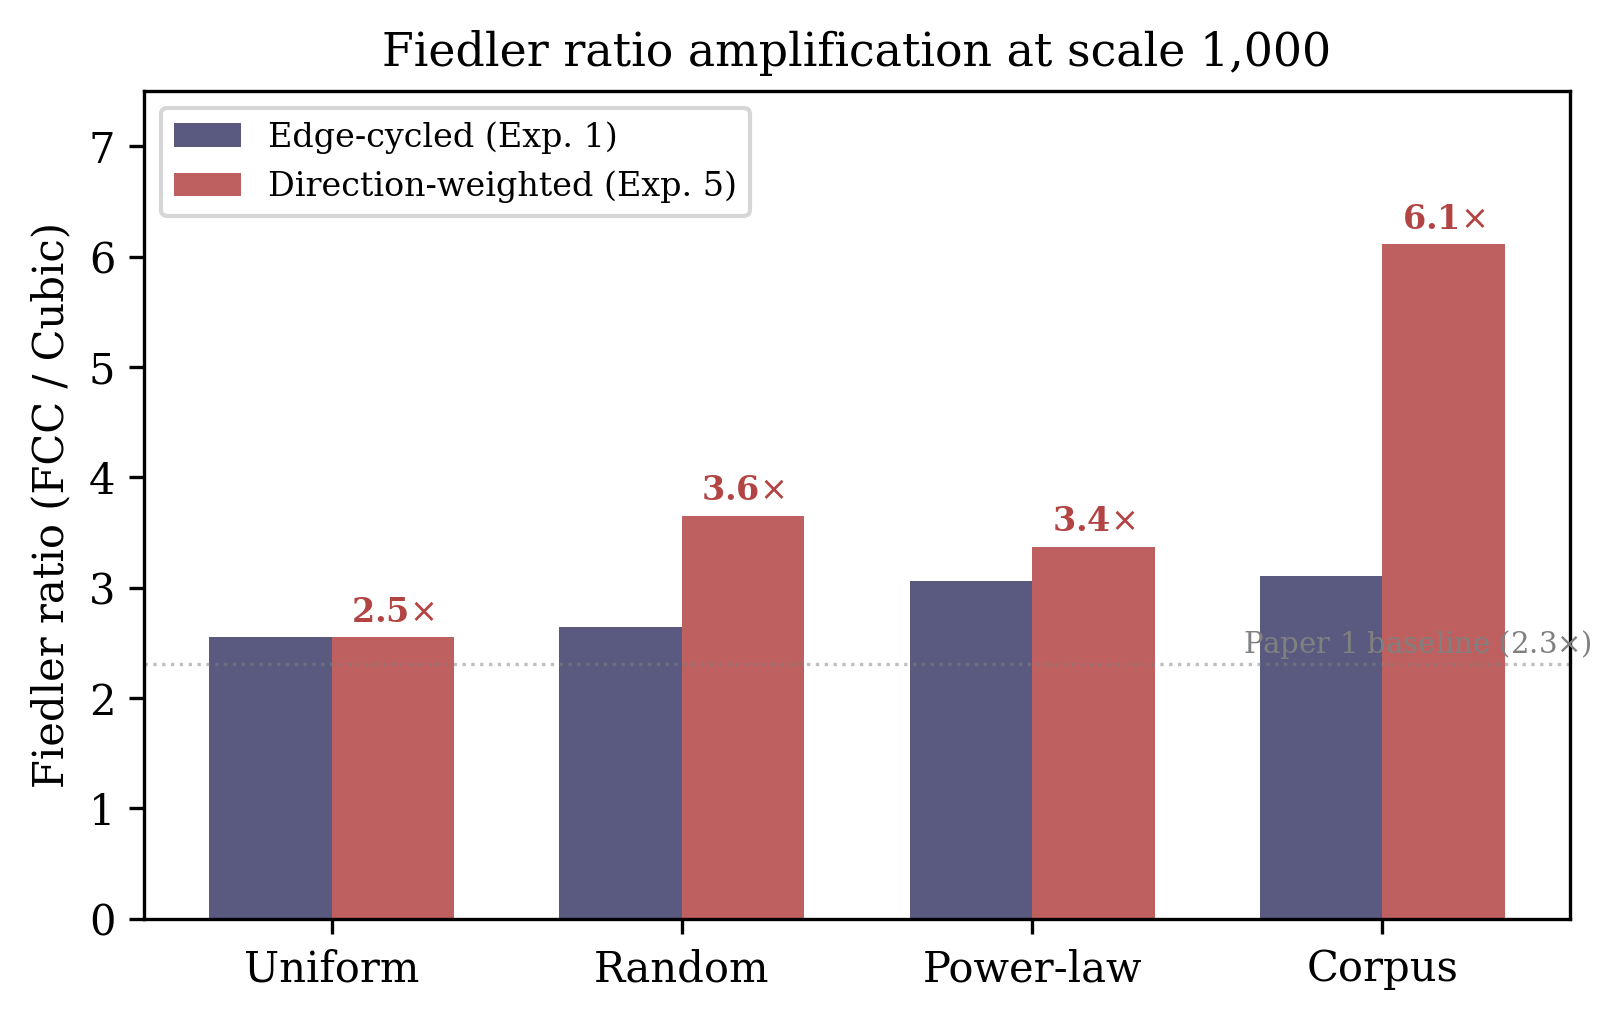
\includegraphics[width=0.75\textwidth]{figures/fig3-amplification-gradient}
\caption{Amplificazione del rapporto di Fiedler a scala 1\,000:
  ciclaggio sugli archi (Esperimento~1) rispetto a ponderazione per
  direzione (Esperimento~5) su quattro distribuzioni di pesi. La linea
  tratteggiata segna la linea di base non pesata dell'Articolo~1
  ($2{,}3\times$). La ponderazione per direzione con valori del corpus
  raggiunge $6{,}1\times$.}
\label{fig:amplification}
\end{figure}

\paragraph{Controllo per permutazione.} Per confermare che
l'amplificazione \`e determinata dall'allineamento dei pesi ordinati con
le coppie di direzioni---e non semplicemente dall'avere 6 raggruppamenti
rispetto a 3---abbiamo eseguito 1\,000 prove in cui i 24 valori del
corpus sono stati permutati casualmente prima della fase di
raggruppamento ordinato a scala 1\,000. Il rapporto di Fiedler medio
permutato \`e stato $2{,}68 \pm 0{,}68$, rispetto a $6{,}11$ per
l'assegnazione ordinata ($p = 0{,}001$). L'assegnazione ordinata
concentra i valori estremi in canali direzionali coerenti, massimizzando
il contrasto ai colli di bottiglia che la connettivit\`a ridondante
dell'FCC sfrutta.

\subsection{Il meccanismo di amplificazione}

Perch\'e la ponderazione per direzione amplifica pi\`u del ciclaggio
sugli archi?

Il ciclaggio sugli archi distribuisce i pesi quasi casualmente tra le
direzioni, diluendo l'effetto collo di bottiglia. La ponderazione per
direzione assegna lo \emph{stesso} peso a tutti gli archi di una coppia
di direzioni. Una coppia di direzioni pesante crea un percorso
uniformemente rafforzato attraverso il reticolo; una coppia leggera ne
crea uno uniformemente indebolito. La coppia di direzioni pi\`u debole
diventa il collo di bottiglia. L'FCC ha 6 coppie di direzioni, quindi
rimuovendo la pi\`u debole restano ancora 5 percorsi alternativi. L'SC
ha 3 coppie di direzioni, quindi la coppia pi\`u debole rappresenta un
terzo di tutta la connettivit\`a.

La metrica del consenso rivela un effetto dipendente dalla scala
(Figura~\ref{fig:consensus}). A scala 125, la pi\`u ricca connettivit\`a
locale dell'FCC domina: il consenso con corpus converge $6{,}69\times$
pi\`u velocemente. A scala 1\,000, il vantaggio si inverte a
$0{,}73\times$ (cubico pi\`u veloce). L'inversione si verifica perch\'e
la media laplaciana divide l'aggiornamento di ciascun nodo per il suo
grado ($1/13$ per i nodi interni FCC, $1/7$ per SC). A scala ridotta,
la connettivit\`a pi\`u ricca compensa; a scala maggiore, la diluizione
per vicino domina. Ci\`o corrisponde al risultato non pesato
dell'Articolo~1~\cite{bielec2026shape} e ne conferma la natura
strutturale.

\begin{figure}[H]
\centering
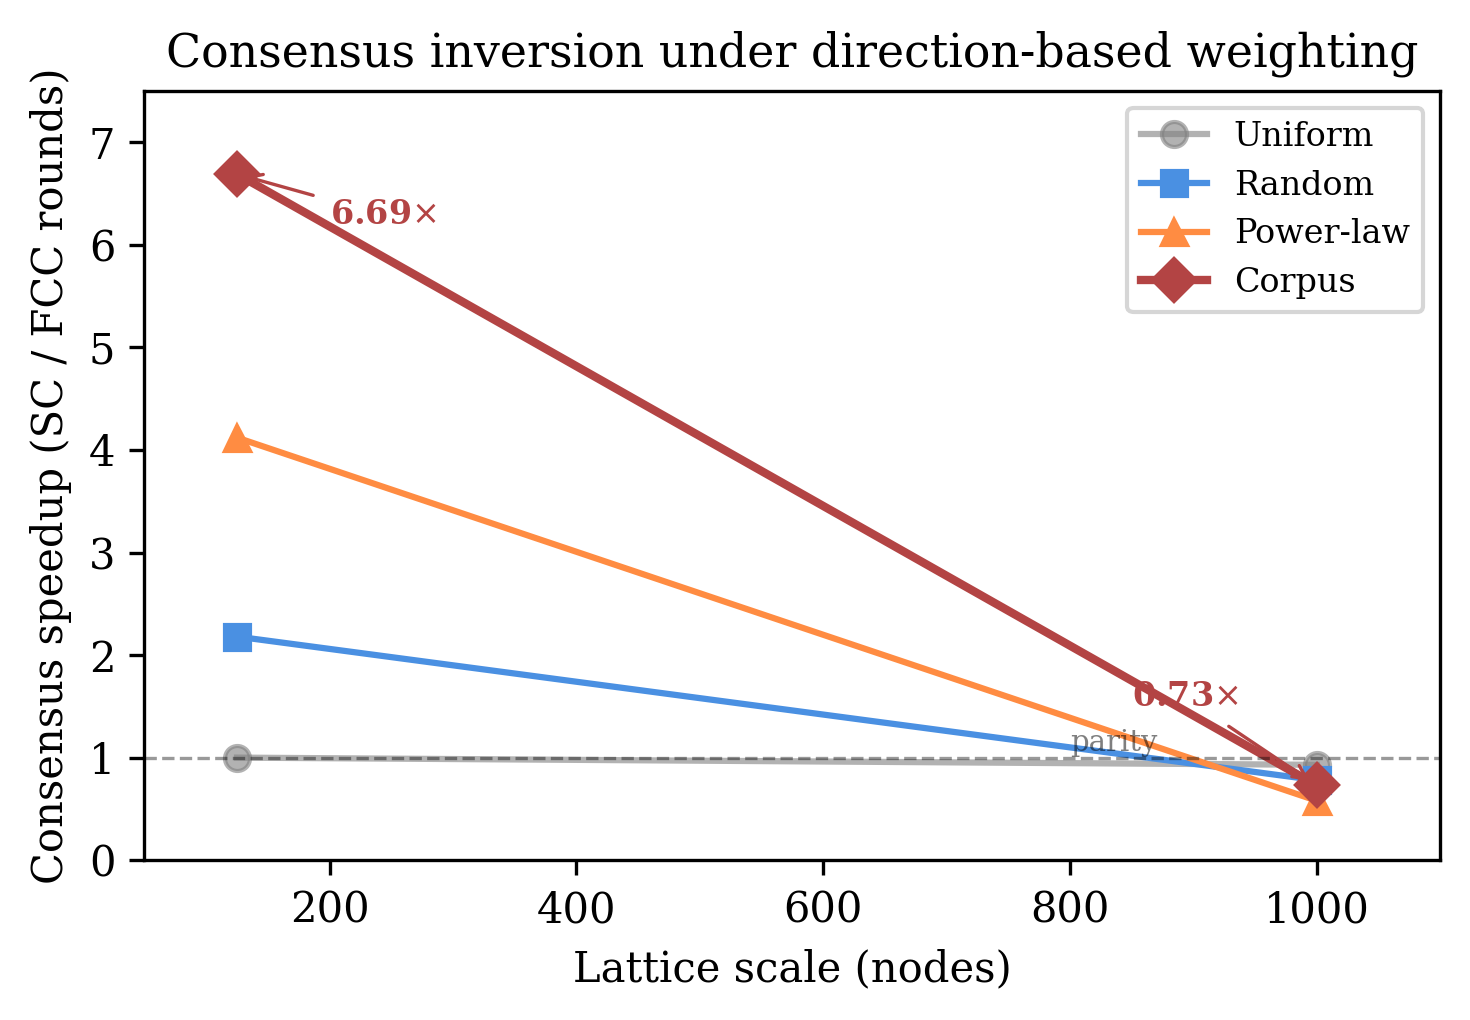
\includegraphics[width=0.7\textwidth]{figures/fig4-consensus-inversion}
\caption{Accelerazione del consenso (cicli SC/FCC, ${>}\,1$ = FCC pi\`u
  veloce) sotto ponderazione per direzione alle scale 125 e 1\,000.
  I pesi del corpus producono un vantaggio FCC di 6,69$\times$ a scala
  125, che si inverte a 0,73$\times$ a scala 1\,000. La transizione tra
  il vantaggio di connettivit\`a locale e il costo di diluizione per
  vicino \`e strutturale.}
\label{fig:consensus}
\end{figure}

% ===================================================================
\section{Caratterizzazione a singola cella}
\label{sec:cell}

\subsection{Esperimento 2: Assegnazione ottimale sul dodecaedro rombico}

I 24 valori del corpus sono assegnati ai 24 archi del dodecaedro
rombico (14 vertici, 24 archi) per minimizzare la variazione totale
(TV)---la somma delle differenze assolute su tutti gli archi a ciascun
vertice. L'ottimizzazione utilizza il ricottura
simulata~\cite{kirkpatrick1983} con 100 riavvii di 5\,000 iterazioni
ciascuno.

\begin{table}[H]
\centering
\caption{Minimizzazione della TV sul dodecaedro rombico. Media casuale
  da 10\,000 assegnazioni casuali. Controllo: un grafo casuale a 24
  archi su 14 vertici.}
\label{tab:exp2}
\begin{tabular}{lrrrr}
\toprule
Distribuzione & TV ottimale & TV media casuale & Miglioramento & $p$-value \\
\midrule
casuale    & 8,71 & 17,73 $\pm$ 1,22 & 50,9\% & ${\leq}\,10^{-4}$ \\
legge di potenza & 6,89 & 10,08 $\pm$ 0,50 & 31,7\% & ${\leq}\,10^{-4}$ \\
corpus    & 8,12 & 13,05 $\pm$ 0,74 & 37,8\% & ${\leq}\,10^{-4}$ \\
\midrule
\multicolumn{5}{l}{\textit{Controllo: grafo casuale a 24 archi}} \\
corpus    & 6,80 & --- & --- & --- \\
\bottomrule
\end{tabular}
\end{table}

La struttura bipartita del dodecaedro rombico (ogni arco connette un
vertice di grado~3 a un vertice di grado~4) vincola piuttosto che
ottimizzare l'assegnazione: un grafo casuale a 24 archi raggiunge
TV~=~6,80 sui valori del corpus rispetto agli 8,12 del DR. Il vincolo
bipartito impone un costo strutturale sull'ordinamento, non un
vantaggio---e questo stesso vincolo \`e ci\`o che produce la
tassellazione 12-connessa.

\subsection{Esperimento 3: Coerenza con i primi (modello nullo onesto)}

L'assegnazione ottimale degli archi dall'Esperimento~2 \`e valutata per
la divisibilit\`a per numeri primi sugli 8 vertici trivalenti: per
ciascun vertice, si conta il numero di archi il cui peso \`e divisibile
per il primo assegnato a quel vertice. Il punteggio di coerenza ottimale
\`e 7 contro una media nulla di $6{,}06 \pm 0{,}85$ ($p = 0{,}30$).

Questo test \`e sottodimensionato: 8 vertici, 24 archi, 8 primi---lo
spazio combinatorio \`e troppo ridotto perch\'e 8 primi si separino dal
rumore utilizzando un semplice conteggio di divisibilit\`a. Il risultato
ha motivato la riprogettazione nell'Esperimento~6, che pone la domanda
corretta attraverso una ricerca esaustiva dello spazio delle mappature.

\subsection{Esperimento 4: Propriet\`a spettrali}

Lo spettro del laplaciano pesato del dodecaedro rombico sotto quattro
distribuzioni rivela il meccanismo alla base dell'amplificazione
dell'Esperimento~1.

\begin{table}[H]
\centering
\caption{Propriet\`a spettrali del DR sotto quattro distribuzioni di
  pesi. Percentile di Fiedler del corpus calcolato rispetto a 10\,000
  prove con pesi casuali.}
\label{tab:exp4}
\begin{tabular}{lrrrr}
\toprule
Distribuzione & Fiedler & Gap spettrale & $\lambda_{\max}$ & Distinti / 14 \\
\midrule
uniforme    & 1,4384 & 0,2055 & 7,0000 & 6 \\
casuale     & 0,5364 & 0,1126 & 4,7654 & 14 \\
legge di potenza  & 0,1041 & 0,0371 & 2,8073 & 14 \\
corpus     & 0,0863 & 0,0314 & 2,7547 & 14 \\
\midrule
\multicolumn{5}{l}{Percentile di Fiedler del corpus vs.\ 10K pesi casuali: \textbf{0,08\%}} \\
\bottomrule
\end{tabular}
\end{table}

Emergono due risultati. Primo, i pesi del corpus sopprimono il valore
di Fiedler allo 0,08-esimo percentile---prossimit\`a alla
disconnessione. Ci\`o identifica il meccanismo: i valori del corpus
creano colli di bottiglia che il reticolo cubico non riesce ad aggirare.
I cammini addizionali dell'FCC forniscono alternative, producendo un
\emph{rapporto} di Fiedler amplificato anche se il valore assoluto di
Fiedler diminuisce.

Secondo, i pesi del corpus rompono tutte le degenerazioni degli
autovalori (Figura~\ref{fig:spectra}). Lo spettro uniforme del DR
presenta solo 6 autovalori distinti su 14 (alta degenerazione dalla
simmetria $O_h$); i pesi del corpus li separano tutti e 14. La rottura
della degenerazione sotto perturbazione \`e un indicatore di quanta
``informazione'' la perturbazione trasporta rispetto alla simmetria del
grafo. I valori del corpus trasportano informazione massimale per il DR.

\begin{figure}[H]
\centering
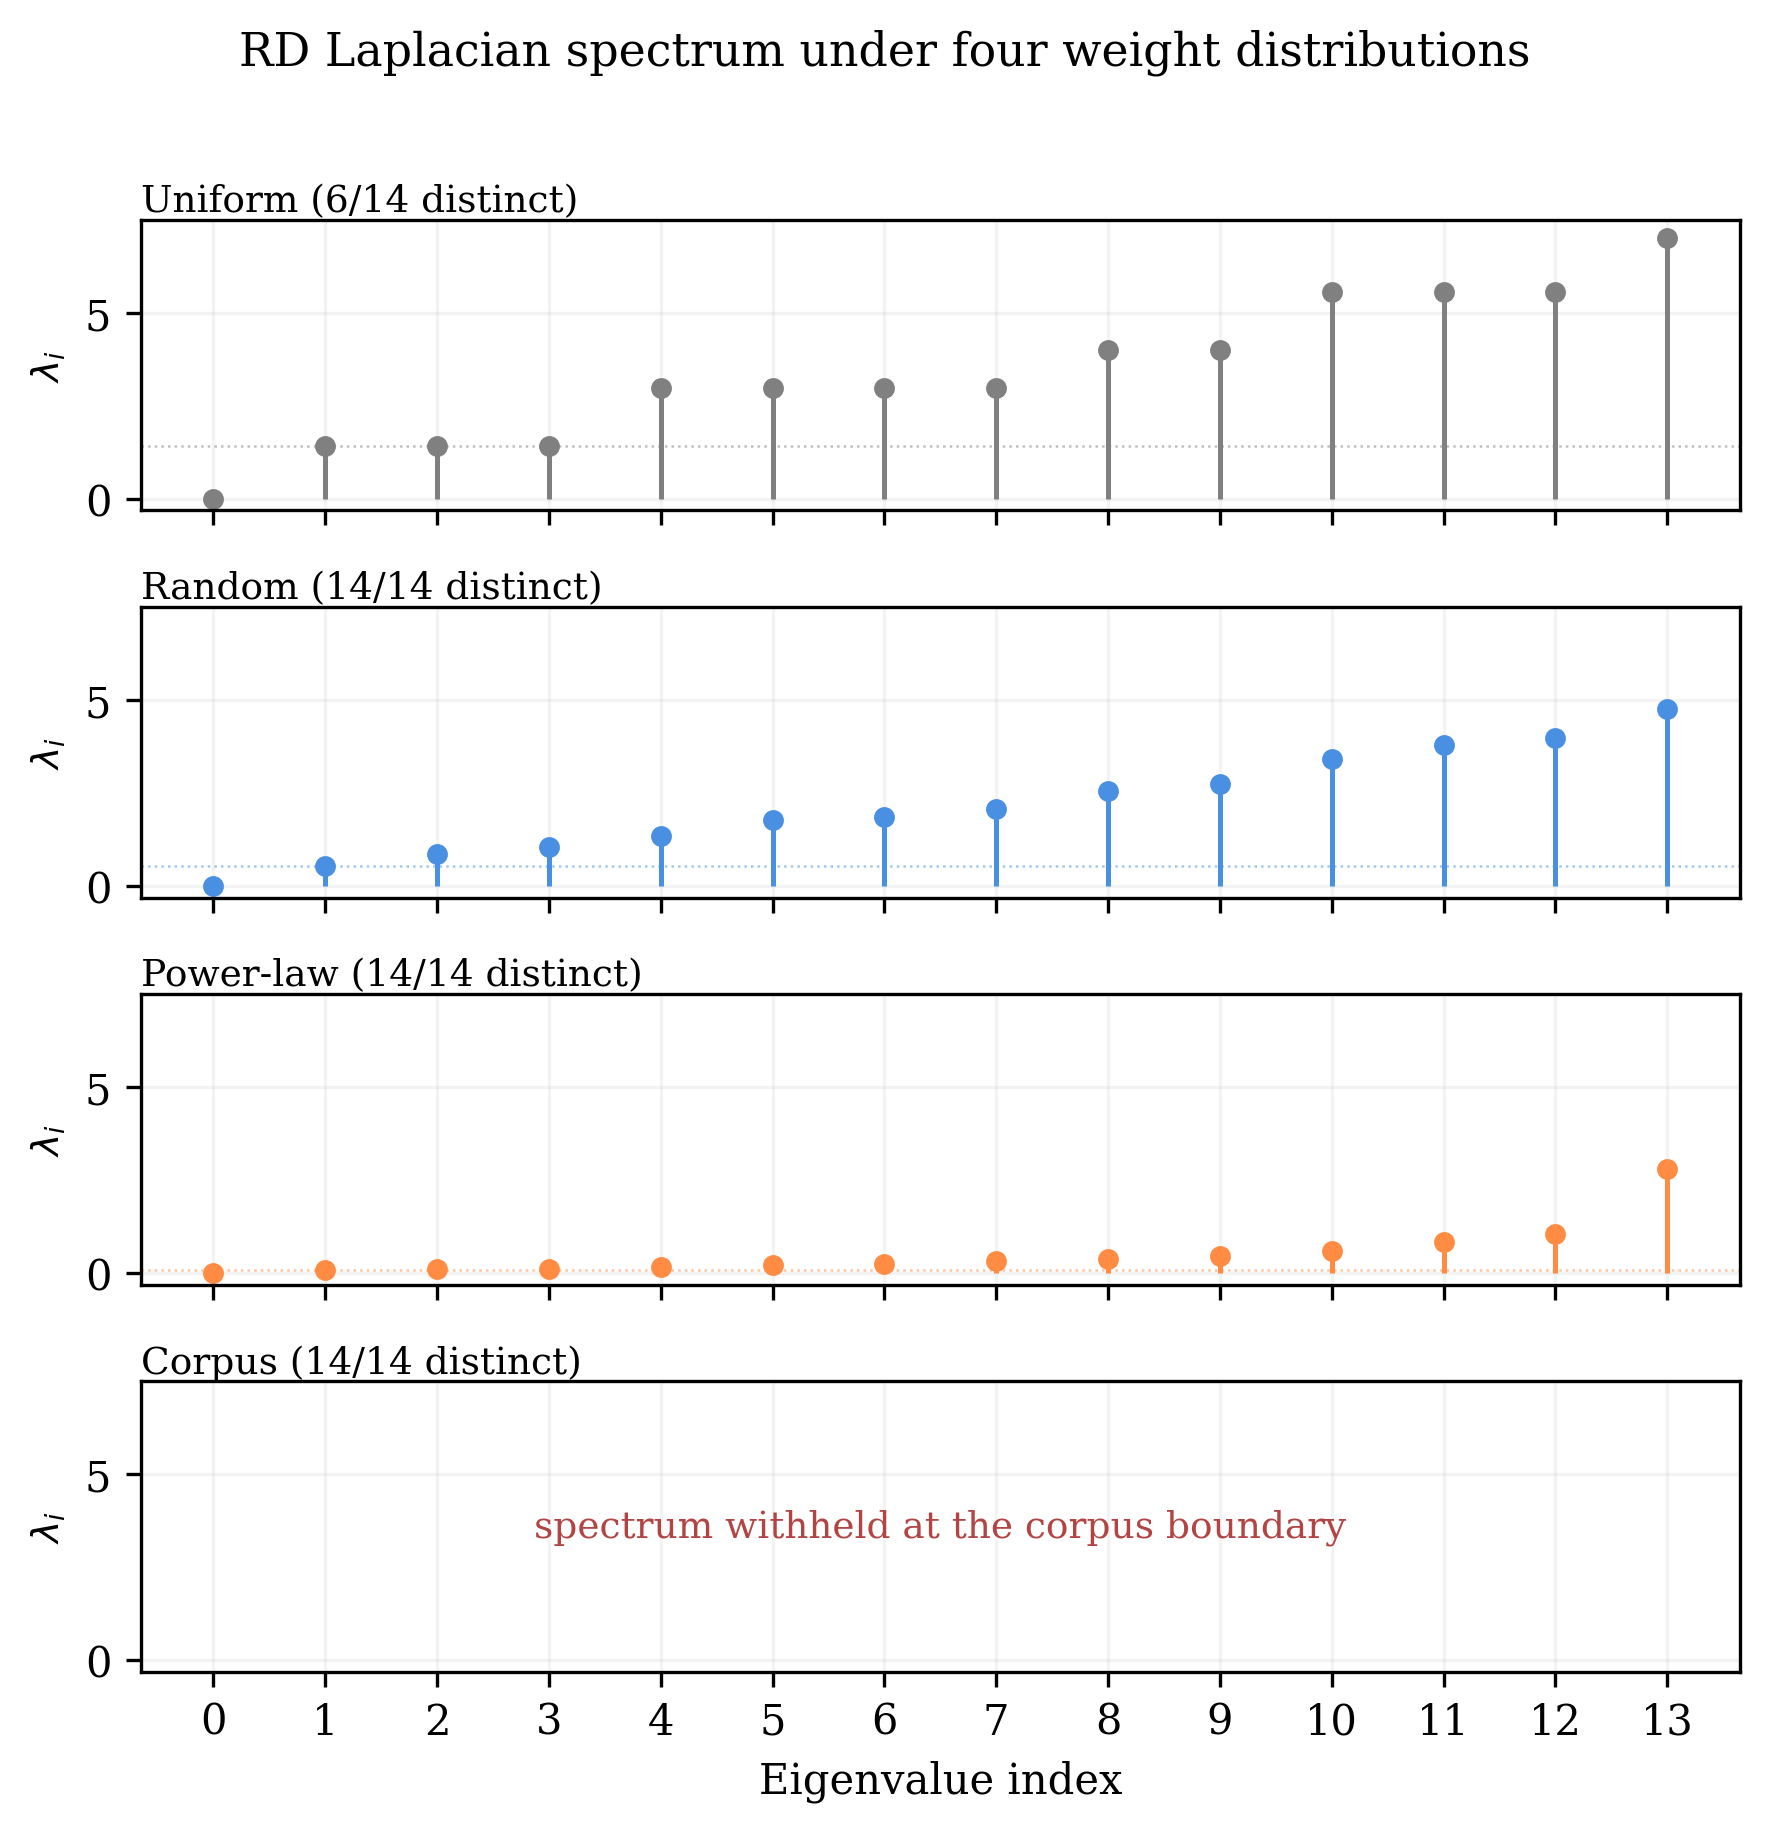
\includegraphics[width=0.85\textwidth]{figures/fig5-spectral-stems}
\caption{Spettri del laplaciano pesato del dodecaedro rombico sotto
  quattro distribuzioni. Le linee orizzontali tratteggiate indicano il
  valore di Fiedler ($\lambda_2$). I pesi uniformi producono 6
  autovalori distinti (alta degenerazione); i pesi del corpus rompono
  tutte le 14 degenerazioni.}
\label{fig:spectra}
\end{figure}

\subsection{Esperimento 6: Mappatura mirata primo-vertice (esplorativa)}

Questo esperimento \`e esplorativo: esplora un paesaggio di
ottimizzazione derivato e va interpretato come analisi strutturata dei
dati piuttosto che come test confermativo di ipotesi. La rubrica di
punteggio \`e stata progettata per catturare livelli multipli di
divisibilit\`a per numeri primi; scelte diverse della rubrica
produrrebbero mappature ottimali e $p$-value differenti.

Data l'assegnazione ottimale degli archi dall'Esperimento~2, si
esaminano esaustivamente tutte le $8! = 40\,320$ mappature degli 8
primi tracciati sugli 8 vertici trivalenti. Ogni mappatura \`e valutata
con una rubrica a tre livelli: divisibilit\`a diretta (un valore di arco
al vertice \`e divisibile per il primo assegnato, peso~3),
divisibilit\`a per somma/differenza (una somma o differenza tra coppie
di valori di arco \`e divisibile, peso~2) e fattori primi condivisi (un
valore di arco condivide un fattore primo con il primo assegnato,
peso~1).

\begin{table}[H]
\centering
\caption{Mappatura primo-vertice: ottimale rispetto a identit\`a e
  modello nullo. Enumerazione esaustiva di tutte le 40\,320
  permutazioni.}
\label{tab:exp6}
\begin{tabular}{lrrr}
\toprule
Mappatura & Punteggio & $p$-value & Rango \\
\midrule
\textbf{Ottimale} (determinata dalla geometria) & \textbf{35,0} & $\mathbf{2{,}5 \times 10^{-5}}$ & 1 / 40\,320 \\
Identit\`a (primo$[i] \to$ vertice$[i]$) & 20,0 & 0,46 & 15\,135 / 40\,320 \\
Media nulla & 19,5 $\pm$ 3,6 & --- & --- \\
\bottomrule
\end{tabular}
\end{table}

La mappatura ottimale \`e la singola permutazione con il punteggio
pi\`u alto su tutte le $8! = 40\,320$ prove
($p \approx 1/40\,320 = 2{,}5 \times 10^{-5}$). Cinque degli otto primi
presentano riscontri di divisibilit\`a diretta nella stella del vertice
assegnato:
\begin{itemize}
  \item $67 \to$ vertice 7: un arco $= 2 \times 67$
  \item $29 \to$ vertice 0: un arco $= 15 \times 29$
  \item $19 \to$ vertice 4: un arco $= 7 \times 19$
  \item $17 \to$ vertice 3: un arco $= 8 \times 17$
  \item $11 \to$ vertice 5: un arco $= 5 \times 11$
\end{itemize}

La mappatura identit\`a---l'ordinamento determinato dall'analisi del
corpus sorgente (primo$[i]$ assegnato al vertice $i$ in ordine di
indice)---ottiene un punteggio pari alla media nulla ($p = 0{,}46$).
L'ordinamento del corpus non si trasferisce agli indici dei vertici.
La geometria richiede la propria disposizione, e tale disposizione \`e
significativa.

\subsection{Esperimento 7: Confronto spettrale tra politopi}

Cinque grafi con 24 archi sono confrontati sotto pesi del corpus per
verificare se gli effetti spettrali osservati nell'Esperimento~4 sono
specifici del dodecaedro rombico.

\begin{table}[H]
\centering
\caption{Cinque grafi a 24 archi sotto pesi del corpus. Percentile
  calcolato rispetto a 10\,000 prove con pesi casuali per grafo.
  Degenerazione: autovalori distinti sotto pesi uniformi / del corpus.}
\label{tab:exp7}
\begin{tabular}{lrrrrr}
\toprule
Grafo & $|V|$ & $\lambda_2$ uniforme & $\lambda_2$ corpus & Percentile & Degen.\ (U/C) \\
\midrule
DR               & 14 & 1,4384 & 0,0863 & 0,08\% & 6 / 14 \\
Cubottaedro    & 12 & 2,0000 & 0,1347 & 0,02\% & 4 / 12 \\
$K_{4,6}$        & 10 & 4,0000 & 0,3886 & 0,36\% & 4 / 10 \\
3-regolare        & 16 & 0,4565 & 0,0538 & 1,04\% & 15 / 16 \\
Casuale $G(14,24)$ & 14 & 0,6997 & 0,0529 & 5,94\% & 14 / 14 \\
\bottomrule
\end{tabular}
\end{table}

La soppressione del valore di Fiedler con pesi del corpus si verifica
in tutti e cinque i grafi a 24 archi testati
(Figura~\ref{fig:polytopes}). Il cubottaedro mostra una soppressione
ancora pi\`u marcata (0,02\%) rispetto al DR (0,08\%). I grafi ad alta
simmetria (DR, cubottaedro, $K_{4,6}$) mostrano la massima rottura
delle degenerazioni sotto pesi del corpus. Ci\`o suggerisce che gli
effetti spettrali sono determinati principalmente dalla distribuzione
dei pesi del corpus---alta varianza e coda pesante che creano colli di
bottiglia---piuttosto che da un'interazione specifica con la topologia
del DR.

\begin{figure}[H]
\centering
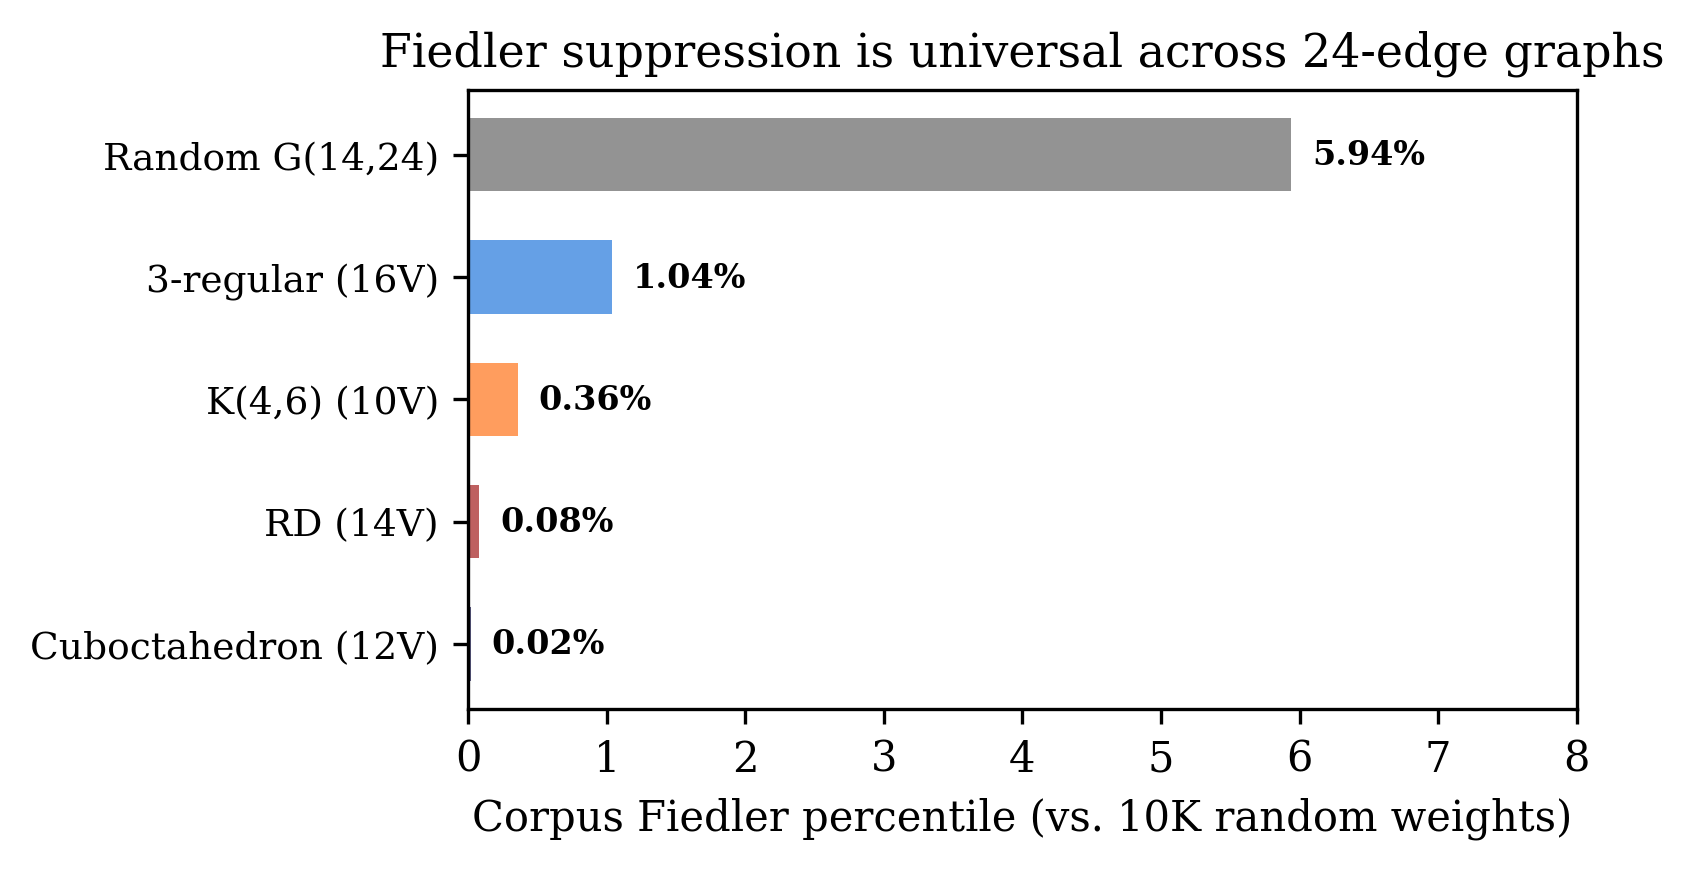
\includegraphics[width=0.75\textwidth]{figures/fig6-polytope-percentiles}
\caption{Percentile di Fiedler del corpus (vs.\ 10K pesi casuali)
  su cinque grafi a 24 archi. La soppressione \`e coerente su tutti i
  grafi testati; il cubottaedro \`e il caso pi\`u estremo. I grafi ad
  alta simmetria si raggruppano ai percentili pi\`u bassi.}
\label{fig:polytopes}
\end{figure}

Ci\`o che \emph{\`e} specifico del DR \`e che esso tassella
$\mathbb{R}^3$. Il cubottaedro, il $K_{4,6}$ e il grafo 3-regolare
non lo fanno. La sensibilit\`a spettrale \`e una propriet\`a dei
valori; l'amplificazione a scala di reticolo \`e una propriet\`a della
topologia. Il DR \`e l'unico grafo in questo confronto che produce
entrambe.

% ===================================================================
\section{Discussione}
\label{sec:discussion}

\subsection{Il meccanismo di amplificazione}

I due esperimenti a scala di reticolo stabiliscono un meccanismo
chiaro. Pesi eterogenei creano colli di bottiglia: archi o coppie di
direzioni con peso basso che vincolano il flusso attraverso il
reticolo. Il valore di Fiedler pesato $\lambda_2(L_w)$ \`e governato
dal collo di bottiglia peggiore del grafo---la direzione di taglio con
la conduttanza pi\`u bassa.

Nel reticolo SC, ciascuna delle 3 coppie di direzioni rappresenta un
terzo di tutta la connettivit\`a. Una coppia di direzioni debole
elimina un terzo di tutti i cammini. Nel reticolo FCC, ciascuna delle
6 coppie di direzioni rappresenta un sesto. Una coppia di direzioni
debole elimina solo un sesto, e le restanti 5 coppie forniscono
cammini alternativi. Il rapporto di connettivit\`a residua ($5/6$
vs.\ $2/3$) si compone attraverso il reticolo, producendo
l'amplificazione osservata da $2{,}3\times$ a $6{,}1\times$.

Il ciclaggio sugli archi (Esperimento~1) raggiunge un'amplificazione
pi\`u modesta (fino a $3{,}2\times$) perch\'e distribuisce i pesi
quasi casualmente tra le direzioni, annullando parzialmente l'effetto
collo di bottiglia all'interno di ciascuna coppia di direzioni.

\subsection{Perch\'e funziona la ponderazione per direzione}

La ponderazione per direzione non \`e una scelta arbitraria. La cella
di Voronoi del reticolo FCC---il dodecaedro rombico---ha 12 facce in
6 coppie parallele. Ogni coppia definisce una direzione attraverso il
reticolo. Ponderare per coppia di direzioni rispetta questa struttura
geometrica: rende ciascun ``canale'' attraverso il reticolo
uniformemente forte o debole, massimizzando il contrasto tra canali
e quindi massimizzando l'effetto collo di bottiglia che la
connettivit\`a ridondante dell'FCC pu\`o superare.

Si tratta di una forma di \emph{risonanza strutturale}: l'assegnazione
dei pesi si allinea con la simmetria intrinseca della topologia, e il
vantaggio topologico si compone di conseguenza. Una validazione
indipendente proviene dall'elaborazione del segnale: Fu
et al.~\cite{fu2009rhombic} hanno dimostrato che la mappa del
dodecaedro rombico fornisce uno schema ottimale per la codifica di
video panoramici, superando le proiezioni cubiche in uniformit\`a di
campionamento e distorsione. La loro scoperta che la geometria delle
coppie di facce del DR produce una mappatura superiore dei dati
sferici conferma che il vantaggio spettrale misurato in questa sede
si estende alle applicazioni pratiche di elaborazione del segnale.

\subsection{La singola cella \`e una finestra}

Gli esperimenti a singola cella (2--4, 6--7) caratterizzano l'effetto
dei pesi strutturati sul DR, ma il peso interpretativo ricade sui
risultati a scala di reticolo. Risultati chiave a singola cella:

\begin{itemize}
  \item Il vincolo bipartito del DR limita l'assegnazione ottimale
    (TV~=~8,12 vs.\ 6,80 per un grafo casuale). La struttura bipartita
    impone un costo strutturale, non un vantaggio di ordinamento.
  \item La mappatura primo-vertice ($p \approx 2{,}5 \times 10^{-5}$)
    mostra una reale struttura aritmetica, ma l'ordinamento determinato
    del corpus non si trasferisce alle etichette dei vertici
    ($p = 0{,}46$). La geometria richiede la propria disposizione.
  \item La soppressione del valore di Fiedler con pesi del corpus si
    verifica in tutti i politopi testati. Ci\`o che \`e specifico del
    DR \`e che esso tassella lo spazio e produce il reticolo in cui si
    verifica l'amplificazione.
\end{itemize}

\subsection{Connessioni con la teoria della resilienza delle reti}
\label{sec:resilience}

Il meccanismo di resilienza ai colli di bottiglia ha paralleli nella
teoria della resilienza delle reti~\cite{dorogovtsev2008}. La Legge
della variet\`a necessaria di Ashby~\cite{ashby1956} prevede che un
controllore debba eguagliare la variet\`a delle perturbazioni che
affronta; pesi eterogenei aumentano la variet\`a delle perturbazioni,
e la topologia 12-connessa dell'FCC fornisce pi\`u cammini
alternativi rispetto ai 6 dell'SC. Il Modello di sistema vitale di
Beer~\cite{beer1972} identifica la fragilit\`a assiale come modalit\`a
di guasto: il reticolo SC \`e allineato sugli assi e una singola coppia
di direzioni debole elimina un terzo della connettivit\`a, mentre
l'FCC distribuisce la connettivit\`a su 6 direzioni diagonali. Questi
quadri di riferimento sono interpretativi---suggeriscono \emph{perch\'e}
l'amplificazione misurata si verifica, ma non costituiscono prove
indipendenti.

\begin{table}[H]
\centering
\caption{Riepilogo dell'amplificazione: linea di base dell'Articolo~1
  rispetto al miglior risultato dell'Articolo~2. Scala indicata per
  ciascuna metrica.}
\label{tab:summary}
\begin{tabular}{lrrl}
\toprule
Metrica & Articolo 1 & Articolo 2 & Metodo \\
\midrule
Rapporto di Fiedler      & 2,55$\times$ & 6,11$\times$ & Corpus ponderato per direzione \\
Vantaggio di cammino     & 32\%         & 61\%         & Corpus con ciclaggio sugli archi \\
Accelerazione del consenso  & 0,93$\times$ & 6,69$\times$ & Corpus ponderato per direzione (scala 125) \\
\bottomrule
\end{tabular}
\end{table}

\subsection{Limitazioni e minacce alla validit\`a}

\textbf{Rapporti deterministici, controllo stocastico.} I rapporti di
Fiedler per le distribuzioni uniforme, legge di potenza e corpus sono
deterministici: data l'assegnazione dei pesi e la costruzione del
reticolo, producono valori identici su tutti i seed testati
($n = 100$). La validazione multi-seed conferma esattamente i rapporti
principali (ad es., $6{,}11\times$ corpus a scala 1\,000 su tutti i
100 seed). Solo la distribuzione casuale introduce varianza:
$3{,}94 \pm 0{,}46$ (IC al 95\% $[3{,}23;\; 4{,}90]$) a scala 1\,000
sotto ponderazione per direzione su 100 seed. Le dinamiche di consenso
sono dipendenti dal seed e beneficerebbero di una validazione aggiuntiva
a scale intermedie.

\textbf{Solo tre dimensioni.} I risultati sono specifici ai reticoli
3D. L'estensione a $D_4$ (4D), $E_8$ (8D) o ad altri reticoli a
dimensioni superiori \`e lavoro futuro.

\textbf{Inversione del consenso.} La metrica del consenso si inverte
tra la scala 125 (vantaggio FCC $6{,}69\times$) e la scala 1\,000
(vantaggio cubico $0{,}73\times$). Il punto di transizione e la sua
dipendenza dalla distribuzione dei pesi non sono ancora risolti.

\textbf{Assenza della linea di base BCC.} Il reticolo cubico a corpo
centrato (8-connesso, cella di Voronoi = ottaedro troncato) \`e il
naturale intermedio tra SC (6) e FCC (12). La sua assenza limita la
possibilit\`a di attribuire gli effetti al solo conteggio di
connettivit\`a rispetto all'isotropia.

\textbf{Provenienza del corpus.} La distribuzione corpus presenta una
struttura interna documentata (primi tracciati, relazioni aritmetiche)
derivata da un dominio analitico indipendente. Sebbene venga qui
valutata insieme a distribuzioni standard, un lettore che metta in
discussione la rappresentativit\`a del corpus pu\`o verificare tutti
i risultati a scala di reticolo utilizzando esclusivamente le
distribuzioni casuale e a legge di potenza, che mostrano lo stesso
gradiente di amplificazione (sebbene a magnitudine inferiore).

% ===================================================================
\section{Lavoro futuro}
\label{sec:future}

\subsection{Architetture di apprendimento geometrico}

La struttura a coppie di direzioni suggerisce un'applicazione naturale
agli adattatori a basso rango (LoRA) per modelli linguistici di grandi
dimensioni: una matrice ponte apprendibile con 6 canali che segue la
topologia delle coppie di facce del DR potrebbe aggiungere un
mescolamento inter-rango a costo di parametri trascurabile. I risultati
su questa architettura ``RhombiLoRA'' sono riportati nell'articolo
complementare~\cite{bielec2026bridge}.

\subsection{Strategia di migrazione: dal cubico al DR}
\label{sec:migration}

Un percorso di adozione in tre fasi rispecchia la nucleazione
cristallina FCC:

\begin{enumerate}
  \item \textbf{Cubico puro} (default attuale): 6-connesso, allineato
    sugli assi.
  \item \textbf{Cubico decorato}: aggiungere 6 connessioni diagonali
    per nodo (i ponti ottaedrici), convertendo ogni cella cubica in una
    cella cubottaedrica. Costo: $2\times$ archi. Beneficio: vantaggio
    di instradamento FCC parziale senza ristrutturazione completa del
    reticolo.
  \item \textbf{DR completo}: sostituire l'indirizzamento cubico con il
    reticolo FCC. 12-connesso, isotropo. L'amplificazione completa di
    Fiedler $6{,}1\times$ sotto pesi strutturati.
\end{enumerate}

In termini ingegneristici: mantenere l'infrastruttura cubica esistente
e aggiungere sei connessioni diagonali a ponte per nodo.

\subsection{Confronto con il BCC}

Il reticolo cubico a corpo centrato \`e il controllo mancante. La sua
cella di Voronoi (l'ottaedro troncato, 14 facce) ha 8 vicini alla
distanza minima---intermedi tra SC (6) e FCC (12). Il BCC raggiunge un
campionamento ottimale in 3D per limiti di banda
isotropi~\cite{petersen1962}. Verificare se esso mostra
un'amplificazione pesata intermedia contribuirebbe ad attribuire il
vantaggio dell'FCC al conteggio di connettivit\`a rispetto
all'isotropia.

\subsection{Dinamiche di consenso sotto validazione multi-seed}

I rapporti di Fiedler sono deterministici attraverso i seed, ma le
dinamiche di consenso (che coinvolgono stati iniziali casuali)
beneficerebbero di una validazione multi-seed, in particolare in
prossimit\`a della transizione di inversione.

\subsection{Risoluzione dell'inversione del consenso}

La transizione tra vantaggio FCC nel consenso (scala 125) e vantaggio
cubico (scala 1\,000) necessita di una risoluzione pi\`u fine. Scale
intermedie (250, 500, 750) individuerebbero il punto di incrocio e
determinerebbero se esso dipende dalla distribuzione dei pesi, dal
rapporto dei gradi o dal diametro del grafo.

\subsection{Estensione a quattro dimensioni: il 24-cella e il reticolo $D_4$}

Il dodecaedro rombico \`e la cella di Voronoi del reticolo FCC in 3D.
Il suo analogo in 4D \`e il \textbf{24-cella}---il politopo regolare
auto-duale unico a quattro dimensioni (24 vertici, 96 archi, 96 facce
triangolari, 24 celle ottaedriche)---che \`e la cella di Voronoi del
reticolo $D_4$~\cite{conway1999, coxeter1973}. Il reticolo $D_4$
raggiunge l'impacchettamento reticolare pi\`u denso noto in 4D, con 24
vicini per sito (rispetto agli 8 del reticolo tesserattico/ipercubico).

Il meccanismo di resilienza ai colli di bottiglia documentato in questa
sede prevede un'amplificazione ancora pi\`u forte in 4D: il rapporto
di vicini \`e $24/8 = 3$ (rispetto a $12/6 = 2$ in 3D), fornendo
pi\`u cammini alternativi attorno ai colli di bottiglia pesati. Le 12
coppie di direzioni del 24-cella (rispetto alle 6 del DR)
supporterebbero una ponderazione per direzione pi\`u ricca.
Un'applicazione naturale \`e la \textbf{correzione quantistica degli
errori}, dove i codici reticolari definiti su topologie a pi\`u alta
connettivit\`a presentano soglie di errore superiori sotto intensit\`a
di accoppiamento eterogenee tra qubit---l'analogo quantistico della
resilienza pesata ai colli di bottiglia.

% ===================================================================
\section{Conclusione}
\label{sec:conclusion}

I pesi strutturati sugli archi amplificano il vantaggio topologico del
reticolo FCC. L'amplificazione \`e monotona con l'eterogeneit\`a dei
pesi, raggiunge il massimo sotto ponderazione per direzione (rapporto
di Fiedler $6{,}1\times$, pi\`u del doppio della linea di base
dell'Articolo~1) e deriva dalla resilienza ai colli di bottiglia: la
topologia 12-connessa dell'FCC aggira i colli di bottiglia che
vincolano i reticoli cubici.

A scala di singola cella, i valori del corpus mostrano una reale
struttura aritmetica (coerenza primo-vertice a
$p \approx 2{,}5 \times 10^{-5}$) ma effetti spettrali
inter-topologici (soppressione del valore di Fiedler in tutti i
politopi testati). Ci\`o che \`e specifico del dodecaedro rombico non
\`e la sua risposta spettrale, bens\`\i\ la sua capacit\`a di
tassellare lo spazio---producendo il reticolo in cui si verifica
l'amplificazione. I modelli nulli onesti (Esperimento~3 a
$p = 0{,}30$, mappatura identit\`a a $p = 0{,}46$) sono tanto
importanti quanto i risultati positivi: definiscono i limiti
dell'analisi a singola cella e prevengono eccessi interpretativi.

Per i professionisti: il vantaggio topologico dell'FCC documentato
nell'Articolo~1 non \`e fragile. Sotto i pesi eterogenei che
caratterizzano i sistemi reali, esso \`e amplificato.

\paragraph{Disponibilit\`a.}
Codice sorgente: \url{https://github.com/tasumermaf/rhombic}.\\
Pacchetto: \url{https://pypi.org/project/rhombic/} (v0.3.0, 256 test,
provenienza di pubblicazione affidabile PyPI vincolata al commit
\texttt{c4d2845db20457a91df2065212a5814e12d22e38}).\\
Riproduzione: \texttt{pip install rhombic==0.3.0 \&\& python
scripts/run\_experiments.py} (tutte le operazioni stocastiche con seed 42).\\
Demo interattiva: \url{https://huggingface.co/spaces/timotheospaul/rhombic}.

% ===================================================================
\section*{Ringraziamenti}

L'autore ringrazia Araminta K per la collaborazione in Promptcrafted.
Parti del codice e del manoscritto sono state sviluppate con assistenza
AI (Claude, Anthropic).

% ===================================================================
\bibliographystyle{plainnat}
\bibliography{rhombic-paper2}

\end{document}
